%=====================================================
%====== If you are new to LaTeX, this website ========
%======     will be your new best friend:     ========
%======   http://en.wikibooks.org/wiki/LaTeX  ========
%======   Template created by Jonathan Blair  ========
%=====================================================



%=====================================================
%============ Controls ===============================
%=====================================================

%\documentclass[12pt,letterpaper,onecolumn]{article}
\documentclass[11pt,letterpaper,onecolumn]{article}
%\documentclass[10pt,letterpaper,onecolumn]{article}  % not recommended
%\documentclass[12pt,letterpaper,twocolumn]{article}
%\documentclass[11pt,letterpaper,twocolumn]{article}
%\documentclass[10pt,letterpaper,twocolumn]{article}


\usepackage{amsmath}
\usepackage{graphicx}
\usepackage{url}
\usepackage{textgreek}
\usepackage{float}
\usepackage{booktabs}
\usepackage{subcaption}
%\graphicspath{{path-to-folder-containing-necessary-graphics}{other folder as necessary}}


%=====================================================
%============ \begin{document} =======================
%=====================================================

\begin{document}

%=====================================================
%============ Title ==================================
%=====================================================

\title{\bf Observation of the Behavior of an Emitter Follower Amplifier}
%\title{\Large\bf Larger, Bolded Title}

%=====================================================
%============ Author =================================
%=====================================================
\author{
 Jairo Portillo \\*
  \\*
 PHY 338K Electronic Techniques \\*
 Department of Physics \\*
 The University of Texas at Austin \\*
 Austin, TX 78712, USA
}
\date{May 6, 2016}

%\address{The University of Texas, Austin, Texas, 78712}

\maketitle

%=====================================================
%============ Abstract ===============================
%=====================================================

\begin{abstract}

In this lab, we will explore the behavior of an emitter follower amplifier. We will focus particularly to its voltage, current, and power gains. We will see that there is a large power gain and that $Z_{in} \gg Z_{out}$ which are associated with a current gain. We will also see that the voltage gain of the circuit is close to 1.

\end{abstract}

%=====================================================
%============ Body of the article ==========================
%=====================================================

%=====================================================
%============ Section ==================================
%=====================================================

\section{Preperation}

 In order to prepare for this lab, we must review the behavior of emitter follower amplifiers. The name is given as the output terminal is at the emitter which follows $V_E \approx V_B - 0.7V$. This circuit is useful due to the fact that the input impedance is much greater than the output input impedance. This allows a signal source to drive the load with less power than it would need if it were directly connected to the load. 

\begin{figure}[H]
\begin{subfigure}{.5\textwidth}
  \centering
  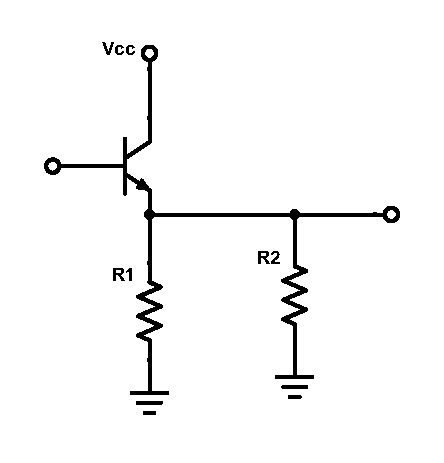
\includegraphics[scale =.6]{Lab-7A.pdf}
  \caption{}
  \label{fig:sub1}
\end{subfigure}%
\begin{subfigure}{.5\textwidth}
  \centering
  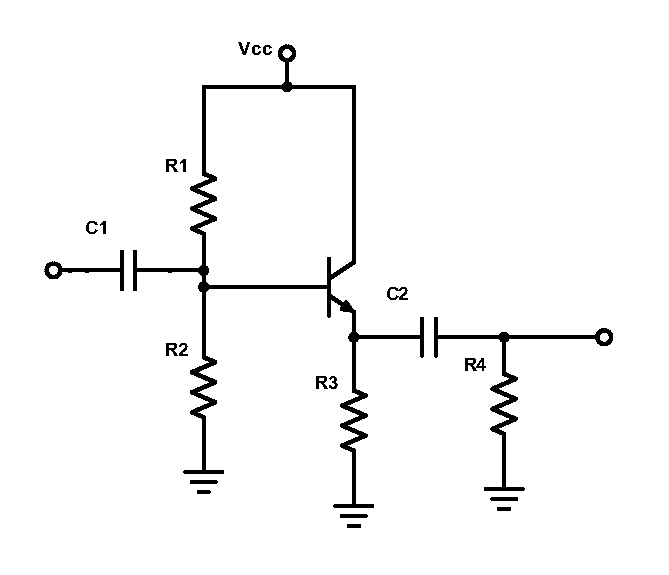
\includegraphics[scale=.5]{Lab-7C.pdf}
  \caption{}
  \label{fig:sub2}
\end{subfigure}
\caption{Emitter Amplifier Circuits}
\label{fig:test}
\end{figure}

We know that for transitors $I_E = I_C + I_B$ and $\beta = \frac{I_C}{I_B}$
thus 
$$I_E = \beta I_B + I_B = \left( 1 + \beta \right) I_B$$
and with $\Delta I_E = \frac{\Delta V_B}{R}$ we can find that
$$\frac{\Delta V_B}{\Delta I_B}= \left( 1 + \beta \right) R = r_{in}$$
or in other words
$$Z_{in} = \left( 1 + \beta \right) Z_{load} \approx \beta Z_{load}$$
and we can find the output impedance to be 
$$Z_{out} = \frac{Z_{source}}{1 + \beta} \approx \frac{Z_{source}}{\beta} $$
with $Z_{in} \gg Z_{out}$. Due to the input and output voltage being approximately the same, there is no voltage gain but there is a power and current gain. The power gain being
$$A_p = \frac{P_{out}}{P_{in}}=\frac{\frac{V_{in}^2}{Z_{in}}}{\frac{V_{out}^2}{Z_{out}}}=\frac{V_{in}^2 Z_{out}}{V_{out}^2 Z_{in}}$$.

\section{Lab work}

\subsection{Data Collection}

We constructed the amplifier circuit with zero base voltage. This caused the transistor to be off and with $V_{CC}= 10V$ we found the output to be 9.8V. In order to obtain a Q point of at 5V, our bias voltage had to be 5.6V. The Voltage gain observed was
$$A_V = \frac{V_{out}}{V_{in}}=\frac{5.28V}{4.8V}=1.1$$

\begin{table}[]
    \centering
    \begin{tabular}{|c|c|}
    \hline
    $Z_{in}$ $\left(k\Omega \right)$ & $V_{out}$  \\ \hline
    10 & 10 \\
    100 & 9.8 \\
    500 & 6.8 \\
    841 & 5.2 \\
    \hline
    \end{tabular}
    \caption{Input impedance and output voltage for an input of 10V}
    \label{tab:my_label}
\end{table}

We then tested the input impedance of the follower and found that at 841 k$\Omega$ , the output is reduced by a factor of 2 and was below our expected 925 k$\Omega$. To test the output impedence we used $C_1 = .48\mu F$, $C_2 = 100\mu F$, 10 k$\Omega$ for the voltage divider. For the power gain, we used a 101.8 k$\Omega$ resistor for the input and a 2.2 k$\Omega$ for the output. The input voltage was 1.92 V and the output voltage was 648 mV. The gave a power gain of 172.47.


\section{Summary and conclusions}

In this lab, we observed how an emitter follower allows a signal source to drive the load with less power than it would need if it were directly connected to the load. We found the voltage gain to be 1.1 which is slight above 1 as expected. Our input impedance was 841 k$\Omega$ which was less than the expected 925k$\Omega$. We found that our power gain was 172.47 which is close to the expected 185.

%=====================================================
%============ Bibliography  ==============================
%=====================================================



%=====================================================
%============ End ====================================
%=====================================================

\end{document}

%=====================================================
%============ End ====================================
%=====================================================